% Copyright 2019 Clara Eleonore Pavillet

% Author: Clara Eleonore Pavillet
% Description: This is an unofficial Oxford University Beamer Template I made from scratch. Feel free to use it, modify it, share it.
% Version: 1.0

\documentclass{beamer}
% Load Packages
\usepackage[utf8]{inputenc}
\usepackage{xcolor}
\usepackage{tikz}
\usetikzlibrary{positioning,calc}
\usepackage{graphicx}
\usepackage{hyperref}
\usepackage{amsmath}
\usepackage{listings}
\usepackage{fontawesome}
\usepackage[T2A]{fontenc}
\usepackage[utf8]{inputenc}
\usepackage[russian]{babel}

% Define Commands
\newcommand*{\ClipSep}{0.06cm} %To adjust footer logo
\newcommand{\E}{\mathrm{e}\,} %\def\I{e} % used to defined e for exp(x), see later what it should be
\newcommand{\ud}{\mathrm{d}}
\lstset{numbers=left, numberstyle=\tiny, stepnumber=1,firstnumber=1,breaklines=true,
    numbersep=5pt,language=Python,
    stringstyle=\ttfamily,
    basicstyle=\footnotesize, 
    showstringspaces=false
}

\usetheme{oxonian}

\title{Лекция 3. Инструменти за Data Science с езика Python - numpy, cupy, scipy, matplotlib. }
\subtitle{\textit{DTSC001 „Прогнозиране чрез анализ на данни I“}}
\titlegraphic{{
\includegraphics[width=5.3cm]{iaps.png}}\hspace{2cm}{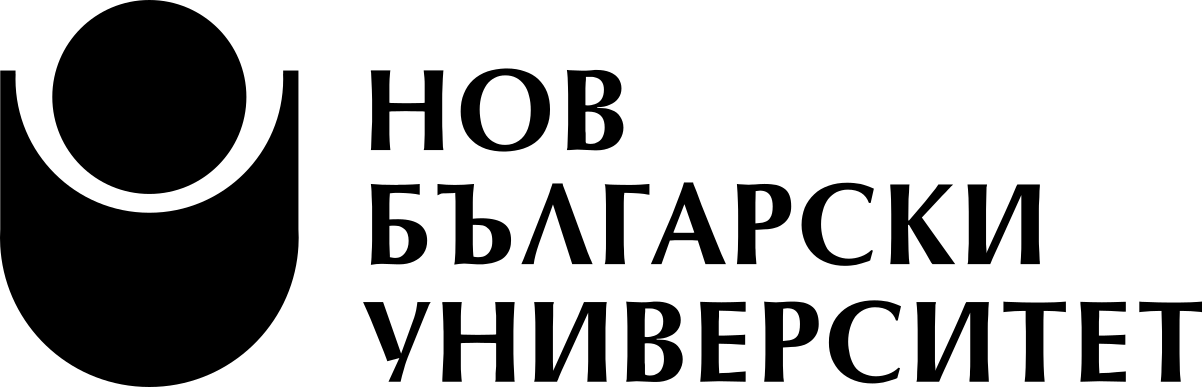
\includegraphics[width=2.5cm]{nbu.png}}} 

\author{\newline \newline \underline{Стоян Мишев}, Лъчезар Петров, Петър Христов}
\institute{\url{https://facebook.com/nbudatascience}}
\date{} %\today

\begin{document}

{\setbeamertemplate{footline}{} 
\frame{\titlepage}}

\section*{План}\begin{frame}{План}\tableofcontents\end{frame}

%\section{Обявления}
%\begin{frame}{Обявления}

%\begin{itemize}
%    \item Д-р Петър Христов ще е в София на 11.01.2020 г. (събота). Той ще може да направи 3 блока от лекции във времевия интервал 13:00 - 18:00. Как е това време за вас?
%    \item  Събиране на ?14.12.2019 (събота)?
%    \begin{itemize}
%        \item за задачи за проекти (СМ + Г. Божиков) - 50 мин.
%        \item презентация на Лъчезар Петров - 30 мин.
%        \item - 
%    \end{itemize}{}
%    
%\end{itemize}{}

%\end{frame}

%\section{Задачи от контролна работа 1}
%\begin{frame}{Задачa 2. Kонтролна работа 1.}
    
%\end{frame}

%\begin{frame}[fragile]{Задачa 1. Kонтролна работа 1.}
%\begin{lstlisting}
%data = pd.read_csv("....csv")
%data.head() 

%#replace all occurences of not available with numpy Nan
%data=data.replace({'Not Available':np.nan})
%for col in list(data.columns):
%    if ('ft²' in col or 'kBtu' in col or 'Metric Tons CO2e' in col or 'kWh' in 
%        col or 'therms' in col or 'gal' in col or 'Score' in col):
%        #convert the data type to float
%        data[col]=data[col].astype(float)
%\end{lstlisting}

%\end{frame}

\section{Numpy}

\begin{frame}[plain]
  \vfill
  \centering
  \begin{beamercolorbox}[sep=8pt,center,shadow=true,rounded=true]{title}
    \usebeamerfont{title}{\insertsectionhead}\par%
    \color{oxfordblue}\noindent\rule{10cm}{1pt} \\
  \end{beamercolorbox}
  \vfill
\end{frame}

\begin{frame}[fragile]{N-мерни масиви}
\begin{verbatim}
>>> import numpy as np
>>> lst = [[1, 2, 3], [4, 5, 6]]
>>> ary2d = np.array(lst)
>>> ary2d
array([[1, 2, 3],
       [4, 5, 6]])
\end{verbatim}
\begin{figure}
    \centering
    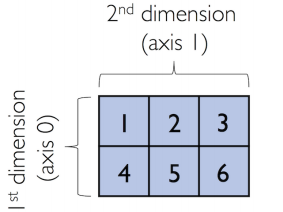
\includegraphics[width=0.32\textwidth]{np1.png}
\end{figure}
\begin{verbatim}
>>> ary2d.dtype
dtype(’int64’)
\end{verbatim}
\end{frame}

\begin{frame}[fragile]{N-мерни масиви}
\begin{verbatim}
>>> float32_ary = ary2d.astype(np.float32)
>>> float32_ary
array([[1., 2., 3.],
[4., 5., 6.]], dtype=float32)
>>> float32_ary.dtype
dtype(’float32’)

>>> ary2d.size
6
>>> ary2d.ndim
2
>>> ary2d.shape
(2, 3)
>>> np.array([1, 2, 3]).shape
(3,)
\end{verbatim}
\end{frame}

\begin{frame}[fragile]{Numpy - dtype, size, ndim, shape, nbytes}
\begin{lstlisting}
arr = np.arange(8).reshape(2,4) #  the total number of elements is unchanged
print(arr)

print('Slicing in the second row:', arr[1, 2:4]) 
print('All rows, third column   :', arr[:, 2])
print('First row:  ', arr[0])
print('Second row: ', arr[1])

print('Data type                :', arr.dtype)
print('Total number of elements :', arr.size)
print('Number of dimensions     :', arr.ndim)
print('Shape (dimensionality)   :', arr.shape)
print('Memory used (in bytes)   :', arr.nbytes)
\end{lstlisting}

\end{frame}

\begin{frame}[fragile]{Създаване нa NumPy масиви}
\begin{verbatim}
>>> np.ones((3, 3))
array([[1., 1., 1.],
       [1., 1., 1.],
       [1., 1., 1.]])
>>> np.zeros((3, 3))
array([[0., 0., 0.],
       [0., 0., 0.],
       [0., 0., 0.]])
>>> np.eye(3)
array([[1., 0., 0.],
       [0., 1., 0.],
       [0., 0., 1.]])
>>> np.diag((3, 3, 3))
array([[3, 0, 0],
       [0, 3, 0],
       [0, 0, 3]])
\end{verbatim}
\end{frame}

\begin{frame}[fragile]{Създаване нa NumPy масиви 2}
\begin{lstlisting}
np.zeros(5, float)
np.zeros(3, int)
np.zeros(3, complex)
print('5 ones:', np.ones(5))
a = np.empty(4) # random
a.fill(5.5)
\end{lstlisting}

\end{frame}


\begin{frame}[fragile]{Създаване нa NumPy масиви 3}
\begin{verbatim}
>>> np.arange(4., 10.)
array([4., 5., 6., 7., 8., 9.])

>>> np.arange(5)
array([0, 1, 2, 3, 4])

>>> np.arange(1., 11., 2)
array([1., 3., 5., 7., 9.])

>>> np.linspace(0., 1., num=5)
array([0. , 0.25, 0.5 , 0.75, 1. ])
\end{verbatim}
\end{frame}

\begin{frame}{Задача}
  Намерете сумата на матриците

  \begin{pmatrix}
    1 & 2 & 3\\
    6 & 8 & 9
  \end{pmatrix}
+
  \begin{pmatrix}
    3 & 5 & 6\\
    7 & 4 & 2
  \end{pmatrix}

използвайки \verb+numpy.
\end{frame}

\begin{frame}[fragile]{Индексиране на NumPy масиви}
\begin{verbatim}
>>> ary = np.array([1, 2, 3])
>>> ary[0]
1
>>> ary[:2] # equivalent to ary[0:2]
array([1, 2])
>>> ary = np.array([[1, 2, 3],
... [4, 5, 6]])
>>> ary[0, 0] # upper left
1
\end{verbatim}
\begin{figure}
    \centering
    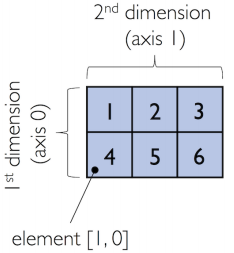
\includegraphics[width=0.35\textwidth]{np2.png}
\end{figure}
\end{frame}

\begin{frame}[fragile]{Индексиране на NumPy масиви 2}
\begin{verbatim}
>>> ary[-1, -1] # lower right
6
>>> ary[0, 1] # first row, second column
2
>>> ary[0] # entire first row
array([1, 2, 3])
>>> ary[:, 0] # entire first column
array([1, 4])
>>> ary[:, :2] # first two columns
array([[1, 2],
[4, 5]])
>>> ary[0, 0]
1
\end{verbatim}
\end{frame}

\begin{frame}{Конструкция на numpy масив}
\begin{figure}
    \centering
    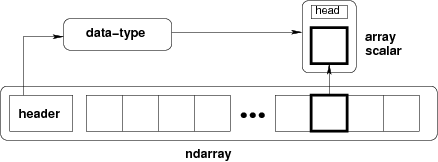
\includegraphics[width=0.7\textwidth]{threefundamental.png}
    \caption{\url{https://docs.scipy.org/doc/numpy-1.13.0/reference/arrays.html}}
    \label{fig:my_label}
\end{figure}{}
\end{frame}

\begin{frame}[fragile]{Ufuncs}
\begin{verbatim}
>>> lst = [[1, 2, 3], [4, 5, 6]]
>>>   for row_idx, row_val in enumerate(lst):
...     for col_idx, col_val in enumerate(row_val):
...        lst[row_idx][col_idx] += 1
>>> lst
[[2, 3, 4], [5, 6, 7]]
>>> lst = [[1, 2, 3], [4, 5, 6]]
>>> [[cell + 1 for cell in row] for row in lst]
>>> ary = np.array([[1, 2, 3], [4, 5, 6]])
>>> ary = np.add(ary, 1)
>>> ary
array([[2, 3, 4],
       [5, 6, 7]])
add, subtract, divide, multiply, and exp
\end{verbatim}
\end{frame}

\begin{frame}[fragile]{Ufuncs 2}
\begin{verbatim}
>>> ary + 1
array([[3, 4, 5],
       [6, 7, 8]])
>>> ary**2
array([[ 4, 9, 16],
       [25, 36, 49]])
       
>>> ary = np.array([[1, 2, 3],
...                 [4, 5, 6]])
>>> np.add.reduce(ary) # column sumns
array([5, 7, 9])
>>> np.add.reduce(ary, axis=1) # row sums
array([ 6, 15])
\end{verbatim}
\end{frame}

\begin{frame}[fragile]{Ufuncs 3}
\begin{verbatim}
>>> ary.sum(axis=0) # column sums
array([5, 7, 9])
>>> ary.sum()
21
\end{verbatim}
\begin{figure}
    \centering
    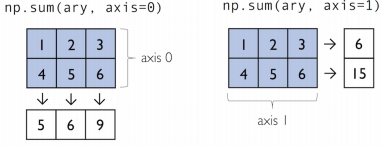
\includegraphics[width=0.55\textwidth]{np3.png}
\end{figure}
\end{frame}

\begin{frame}{Ufunc 4}
• mean (computes arithmetic average)

• std (computes the standard deviation)

• var (computes variance)

• np.sort (sorts an array)

• np.argsort (returns indices that would sort an array)

• np.min (returns the minimum value of an array)

• np.max (returns the maximum value of an array)

• np.argmin (returns the index of the minimum value)

• np.argmax (returns the index of the maximum value)

• array equal (checks if two arrays have the same shape and elements)
\end{frame}

\begin{frame}[fragile]{Broadcasting}
\begin{figure}
    \centering
    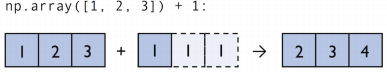
\includegraphics[width=0.55\textwidth]{np5.png}
\end{figure}
\begin{verbatim}
>>> ary1 = np.array([1, 2, 3])
>>> ary2 = np.array([4, 5, 6])
>>> ary1 + ary2
array([5, 7, 9])
>>> ary3 = np.array([[4, 5, 6],
...                  [7, 8, 9]])
>>> ary3 + ary1 # similarly, ary1 + ary3
array([[ 5, 7, 9],
       [ 8, 10, 12]])
\end{verbatim}
\begin{figure}
    \centering
    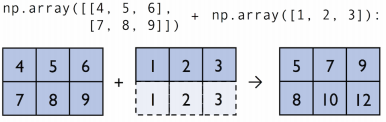
\includegraphics[width=0.55\textwidth]{np6.png}
\end{figure}
\end{frame}

\begin{frame}[fragile]{Индексиране – Memory Views and Copies}
Views
\begin{verbatim}
>>> ary = np.array([[1, 2, 3],
...                 [4, 5, 6]])
>>> first_row = ary[0]
>>> first_row += 99
>>> ary
array([[100, 101, 102],
       [ 4, 5, 6]])
>>> ary = np.array([[1, 2, 3],
... [4, 5, 6]])
>>> first_row = ary[:1]
>>> first_row += 99
>>> ary
array([[100, 101, 102],
[ 4, 5, 6]])
\end{verbatim}
\end{frame}

\begin{frame}[fragile]{Индексиране – Memory Views and Copies}

Views
\begin{verbatim}
>>> ary = np.array([[1, 2, 3],
... [4, 5, 6]])
>>> center_col = ary[:, 1]
>>> center_col += 99
>>> ary
array([[ 1, 101, 3],
[ 4, 104, 6]])
\end{verbatim}
\end{frame}

\begin{frame}[fragile]{Индексиране – Memory Views and Copies}
Copy
\begin{verbatim}
>>> ary = np.array([[1, 2, 3],
... [4, 5, 6]])
>>> second_row = ary[1].copy()
>>> second_row += 99
>>> ary
array([[1, 2, 3],
[4, 5, 6]])
\end{verbatim}
Индексиране
\begin{verbatim}
>>> ary = np.array([[1, 2, 3],
...                 [4, 5, 6]])
>>> ary[:, [0, 2]] # first and and last column
array([[1, 3],
       [4, 6]])
\end{verbatim}
\end{frame}

\begin{frame}[fragile]{Индексиране }
\begin{verbatim}
>>> this_is_a_copy = ary[:, [0, 2]]
>>> this_is_a_copy += 99
>>> ary
array([[1, 2, 3],
       [4, 5, 6]])
>>> ary[:, [2, 0]] # first and and last column
array([[3, 1],
       [6, 4]])
\end{verbatim}
\end{frame}

\begin{frame}[fragile]{Индексиране }
\begin{verbatim}
>>> ary = np.array([[1, 2, 3],
... [4, 5, 6]])
>>> greater3_mask = ary > 3
>>> greater3_mask
array([[False, False, False],
[ True, True, True]])

>>> ary[greater3_mask]
array([4, 5, 6])

>>> ary[(ary > 3) & (ary % 2 == 0)]
array([4, 6])
\end{verbatim}
\end{frame}

\begin{frame}[fragile]{Генератори на случайни числа}
\begin{verbatim}
>>> np.random.seed(123)
>>> np.random.rand(3)
array([0.69646919, 0.28613933, 0.22685145])

>>> rng1 = np.random.RandomState(seed=123)
>>> rng1.rand(3)
array([0.69646919, 0.28613933, 0.22685145])
\end{verbatim}
\end{frame}

\begin{frame}[fragile]{Reshaping Arrays}
\begin{verbatim}
>>> ary1d = np.array([1, 2, 3, 4, 5, 6])
>>> ary2d_view = ary1d.reshape(2, 3)
>>> ary2d_view
array([[1, 2, 3],
       [4, 5, 6]])
>>> np.may_share_memory(ary2d_view, ary1d)
True

>>> ary1d.reshape(2, -1)
array([[1, 2, 3],
[4, 5, 6]])
>>> ary1d.reshape(-1, 2)
array([[1, 2],
[3, 4],
[5, 6]])
\end{verbatim}
\end{frame}

\begin{frame}[fragile]{Reshaping Arrays}
\begin{verbatim}
>>> ary = np.array([[[1, 2, 3],
...                  [4, 5, 6]]])
>>> ary.reshape(-1)
array([1, 2, 3, 4, 5, 6])

>>> ary = np.array([1, 2, 3])
>>> # stack along the first axis
>>> np.concatenate((ary, ary))
array([1, 2, 3, 1, 2, 3])

>>> ary = np.array([[1, 2, 3]])
>>> # stack along the first axis (here: rows)
>>> np.concatenate((ary, ary), axis=0)
array([[1, 2, 3],
[1, 2, 3]])
\end{verbatim}
\end{frame}

\begin{frame}[fragile]{Reshaping Arrays}
\begin{verbatim}
>>> # stack along the second axis (here: column)
>>> np.concatenate((ary, ary), axis=1)
array([[1, 2, 3, 1, 2, 3]])
>>> ary = np.array([[1, 2, 3]])

>>> # stack along the first axis (here: rows)
>>> np.concatenate((ary, ary), axis=0)
array([[1, 2, 3],
       [1, 2, 3]])
\end{verbatim}
\end{frame}

\begin{frame}[fragile]{Comparison Operators and Masks}
\begin{verbatim}
>>> ary = np.array([1, 2, 3, 4])
>>> mask = ary > 2
>>> mask
array([False, False, True, True])
>>> ary[mask]
array([3, 4])
>>> mask
array([False, False, True, True])
>>> mask.sum()
2

>>> np.where(ary > 2, 1, 0)
array([0, 0, 1, 1])
\end{verbatim}
\end{frame}

\begin{frame}[fragile]{Comparison Operators and Masks}
\begin{verbatim}
>>> ary = np.array([1, 2, 3, 4])
>>> mask = ary > 2
>>> ary[mask] = 1
>>> ary[~mask] = 0
>>> ary
array([0, 0, 1, 1])
\end{verbatim}


\begin{verbatim}
• A: & or np.bitwise and
• Or: | or np.bitwise or
• Xor: ^ or np.bitwise xor
• Not: ~ or np.bitwise not
\end{verbatim}

\end{frame}

\begin{frame}[fragile]{Comparison Operators and Masks}
\begin{verbatim}
>>> ary = np.array([1, 2, 3, 4])
>>> (ary > 3) | (ary < 2)

>>> ~((ary > 3) | (ary < 2))
array([False, True, True, False])
\end{verbatim}
\end{frame}

\begin{frame}[fragile]{Линейна алгебра с NumPy масиви}
\begin{verbatim}
>>> row_vector = np.array([1, 2, 3])
>>> row_vector
array([1, 2, 3])

>>> column_vector = np.array([[1, 2, 3]]).reshape(-1, 1)
>>> column_vector
array([[1],
[2],
[3]])

>>> row_vector[:, np.newaxis]
array([[1],
[2],
[3]])
\end{verbatim}
\end{frame}

\begin{frame}[fragile]{Линейна алгебра с NumPy масиви 2 }

\begin{verbatim}
>>> matrix = np.array([[1, 2, 3],
... [4, 5, 6]])
>>> np.matmul(matrix, column_vector)
array([[14],
[32]])
>>> np.matmul(matrix, row_vector)
array([14, 32])
>>> np.matmul(row_vector, row_vector)
14

>>> np.dot(row_vector, row_vector)
14
>>> np.dot(matrix, row_vector)
array([14, 32])

\end{verbatim}
\end{frame}

\begin{frame}[fragile]{Линейна алгебра с NumPy масиви 3 }

\begin{verbatim}
>>> np.dot(matrix, column_vector)
array([[14],
       [32]])

>>> matrix = np.array([[1, 2, 3],
...                    [4, 5, 6]])
>>> matrix.transpose()
array([[1, 4],
    [2, 5],
    [3, 6]])
\end{verbatim}
\begin{figure}
    \centering
    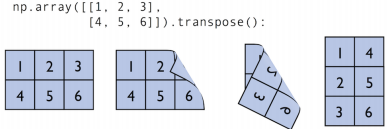
\includegraphics[width=0.55\textwidth]{np9.png}
\end{figure}
\end{frame}
\begin{frame}[fragile]{Линейна алгебра с NumPy масиви 3}
\begin{verbatim}
>>> np.matmul(matrix, matrix.transpose())
array([[14, 32],
[32, 77]])
\end{verbatim}
\begin{figure}
    \centering
%    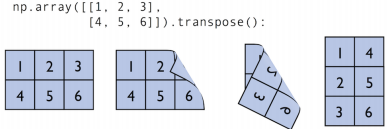
\includegraphics[width=0.55\textwidth]{np9.png}
    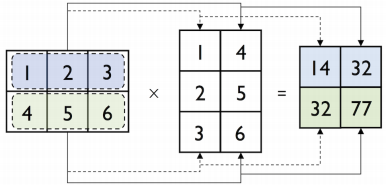
\includegraphics[width=0.55\textwidth]{np10.png}
\end{figure}
\begin{verbatim}
>>> matrix.T
array([[1, 4],
[2, 5],
[3, 6]])
\end{verbatim}
Има и специален тип \verb  matrix  .
\end{frame}


\begin{frame}{Примери от линейната алгебра, решени с NumPy}
    \url{https://www.w3resource.com/python-exercises/numpy/linear-algebra}
\end{frame}

%=================================================


\subsection{NumPy слайдове от 2019/2020}







\begin{frame}[fragile]{Numpy (\url{http://numpy.org}) Двумерен масив}
\begin{lstlisting}
np.arange(1, 100, 5)
print("A linear grid between 0 and 1:", np.linspace(0, 1, 5))
print("A logarithmic grid between 10**1 and 10**4: ", np.logspace(1, 4, 4))
np.random.randn(5) # standard normal distribution
np.random.normal(10, 3, 5)

lst2 = [[1, 2], [3, 4]]
arr2 = np.array([[1, 2], [3, 4]])
print(lst2[0][1])
print(arr2[0,1])

np.array([[1,2,3],[4,5,6]], order='F')
np.zeros((2,3))
np.random.normal(10, 3, (2, 4))
\end{lstlisting}

\end{frame}


\begin{frame}[fragile]{Numpy - min, max, prod, mean, std }

\begin{lstlisting}
print('Minimum and maximum :', arr.min(), arr.max())
print('Sum and product of all elements :', arr.sum(), arr.prod())
print('Mean and standard deviation  :', arr.mean(), arr.std())
\end{lstlisting}

\end{frame}

\begin{frame}[fragile]{Numpy - axis }
\begin{lstlisting}
print('For the following array:\n', arr)
print('The sum of elements along the rows is:', arr.sum(axis=1))
print('The sum of elements along the columns is:', arr.sum(axis=0))

np.zeros((3,4,5,6)).sum(2).shape

print('Array:\n', arr)
print('Transpose:\n', arr.T)
\end{lstlisting}

\end{frame}

\begin{frame}[fragile]{Numpy (\url{http://numpy.org}) }
\begin{lstlisting}
arr1 = np.arange(4)
arr2 = np.arange(10, 14)
print(arr1, '+', arr2, '=', arr1+arr2)
print(arr1, '*', arr2, '=', arr1*arr2)

arr1 + 1.5*np.ones(4)
arr1 + 1.5

b = np.array([2, 3, 4, 5])
print(arr, '\n\n+', b , '\n---------------\n', arr + b)
\end{lstlisting}

\end{frame}

\begin{frame}[fragile]{Numpy (\url{http://numpy.org}) }
\begin{lstlisting}
c = np.array([4, 6])
c[:, np.newaxis]

print(c.shape)
print((c[:, np.newaxis]).shape)

arr + c[:, np.newaxis]

x = np.linspace(0, 2*np.pi, 100)
y = np.sin(x)
\end{lstlisting}

\end{frame}

\begin{frame}[fragile]{Numpy. Матрично умножение.}
\begin{lstlisting}
v1 = np.array([2, 3, 4])
v2 = np.array([1, 0, 1])
print(v1, '.', v2, '=', v1.dot(v2))
print(v1, '.', v2, '=', v1 @ v2)

A = np.arange(6).reshape(2, 3)
print(A, 'x', v1, '=', A @ v1)

print(A @ A.T)

print(A.T @ A)

print(v1, '.', v2, '=', v1 @ v2)

\end{lstlisting}

\end{frame}

\section{CuPy}
\begin{frame}[plain]
  \vfill
  \centering
  \begin{beamercolorbox}[sep=8pt,center,shadow=true,rounded=true]{title}
    \usebeamerfont{title}{\insertsectionhead}\par%
    \color{oxfordblue}\noindent\rule{10cm}{1pt} \\
  \end{beamercolorbox}
  \url{https://cupy.dev/}
  \vfill
\end{frame}


\section{Matplotlib }
\begin{frame}[plain]
  \vfill
  \centering
  \begin{beamercolorbox}[sep=8pt,center,shadow=true,rounded=true]{title}
    \usebeamerfont{title}{\insertsectionhead}\par%
    \color{oxfordblue}\noindent\rule{10cm}{1pt} \\
  \end{beamercolorbox}
  \vfill
\end{frame}

\begin{frame}[fragile]{Matplotlib (\url{https://matplotlib.org/})}
\begin{lstlisting}
import matplotlib.pyplot as plt

x = np.linspace(0, 2*np.pi)
y = np.sin(x)
plt.figure()
plt.plot(x,y, label='sin(x)')
plt.legend()
plt.grid()
plt.title('Harmonic')
plt.xlabel('x')
plt.ylabel('y')

plt.plot(x, y, linewidth=2)

plt.plot(x, y, 'o', markersize=5, color='r');
\end{lstlisting}
\end{frame}

\begin{frame}[fragile]{Matplotlib (\url{https://matplotlib.org/})}
\begin{lstlisting}
mu, sigma = 100, 15
x = mu + sigma * np.random.randn(10000)

# the histogram of the data
n, bins, patches = plt.hist(x, 50, normed=1, facecolor='g', alpha=0.75)

plt.xlabel('Smarts')
plt.ylabel('Probability')
plt.title('Histogram of IQ')
# This will put a text fragment at the position given:
plt.text(55, .027, r'$\mu=100,\ \sigma=15$', fontsize=14)
plt.axis([40, 160, 0, 0.03])
plt.grid()
\end{lstlisting}
\end{frame}

\begin{frame}[fragile]{Matplotlib (\url{https://matplotlib.org/})}
\begin{lstlisting}
from matplotlib import cm

plt.imshow(np.random.rand(5, 10), cmap=cm.gray, interpolation='nearest');

img = plt.imread('stinkbug.png')
print('Dimensions of the array img:', img.shape)
plt.imshow(img);
\end{lstlisting}
\end{frame}


\begin{frame}[fragile]{Matplotlib (\url{https://matplotlib.org/})}
\begin{lstlisting}
from mpl_toolkits.mplot3d.axes3d import Axes3D
from matplotlib import cm

fig = plt.figure()
ax = fig.add_subplot(1, 1, 1, projection='3d')
X = np.arange(-5, 5, 0.25)
Y = np.arange(-5, 5, 0.25)
X, Y = np.meshgrid(X, Y)
R = np.sqrt(X**2 + Y**2)
Z = np.sin(R)
surf = ax.plot_surface(X, Y, Z, rstride=1, cstride=1, cmap=cm.viridis,
        linewidth=0, antialiased=False)
ax.set_zlim3d(-1.01, 1.01);
\end{lstlisting}
\end{frame}



%\section{Бъдещи слайдове}
%\begin{frame}[plain]
%  \vfill
%  \centering
%  \begin{beamercolorbox}[sep=8pt,center,shadow=true,rounded=true]{title}
%    \usebeamerfont{title}{\insertsectionhead}\par%
%    \color{oxfordblue}\noindent\rule{10cm}{1pt} \\
%  \end{beamercolorbox}
%  \vfill
%\end{frame}

%\begin{frame}{SciPy (\url{http://scipy.org})}
%    набор от алгоритми от линейната алгебра, диф. у-ния, интегриране и др.
%\end{frame}



%% \section{Pandas}
%% \begin{frame}[plain]
%%   \vfill
%%   \centering
%%   \begin{beamercolorbox}[sep=8pt,center,shadow=true,rounded=true]{title}
%%     \usebeamerfont{title}{\insertsectionhead}\par%
%%     \color{oxfordblue}\noindent\rule{10cm}{1pt} \\
%%   \end{beamercolorbox}
%%   \vfill
%% \end{frame}

%% \begin{frame}{Pandas}
%%     \begin{itemize}
%%         \item инструменти за работа с данни: reshaping, merging, sorting, slicing, aggregation etc.
%%         \item \textbf{Series} and \textbf{DataFrames} - Series е колона , а DataFrame е многомерна таблица от  Series.
%%     \end{itemize}
%% \begin{figure}
%%     \centering
%%     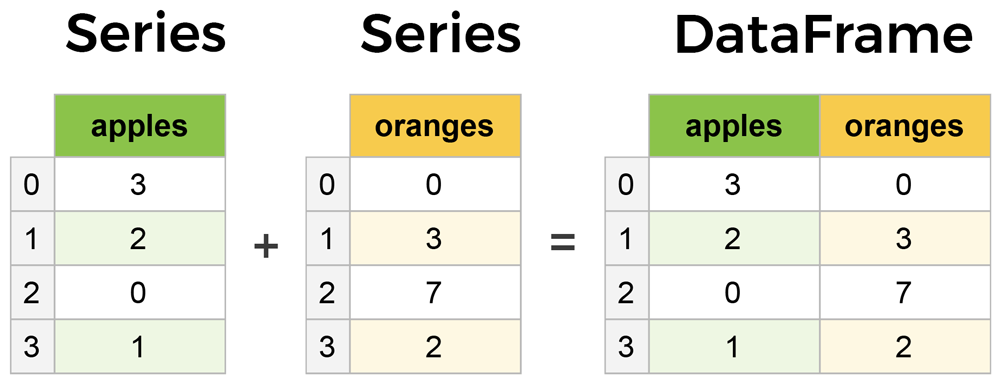
\includegraphics[width=0.7\textwidth]{series-and-dataframe.png}
%% \end{figure}
%% \end{frame}

%% \begin{frame}[fragile]{Pandas}
%% \begin{lstlisting}
%% data = {
%%     'apples': [3, 2, 0, 1], 
%%     'oranges': [0, 3, 7, 2]
%% }
%% purchases = pd.DataFrame(data)

%% purchases = pd.DataFrame(data, index=['June', 'Robert', 'Lily', 'David'])

%% purchases.loc['June']
%% \end{lstlisting}
%% \end{frame}

%% \begin{frame}[fragile]{Pandas}
%% \begin{lstlisting}
%% df = pd.read_json('purchases.json')
%% df = pd.read_sql_query("SELECT * FROM purchases", con)
%% df
%% df.to_csv('new_purchases.csv')
%% df.to_json('new_purchases.json')
%% df.to_sql('new_purchases', con)
%% \end{lstlisting}
%% \end{frame}

%% \begin{frame}[fragile]{Pandas}
%% \begin{lstlisting}
%% movies_df = pd.read_csv("IMDB-Movie-Data.csv", index_col="Title")
%% movies_df.head()
%% movies_df.tail(2)
%% movies_df.info()
%% movies_df.shape
%% \end{lstlisting}
%% \end{frame}


%% \begin{frame}[fragile]{Pandas}
%% \begin{lstlisting}
%% temp_df = movies_df.append(movies_df)
%% temp_df.shape
%% temp_df = temp_df.drop_duplicates()
%% temp_df.shape

%% temp_df.drop_duplicates(inplace=True)

%% temp_df = movies_df.append(movies_df)  # make a new copy

%% temp_df.drop_duplicates(inplace=True, keep=False)

%% temp_df.shape

%% movies_df.columns


%% \end{lstlisting}
%% \end{frame}

%% \begin{frame}[fragile]{Pandas - rename}
%% \begin{lstlisting}
%% movies_df.rename(columns={
%%         'Runtime (Minutes)': 'Runtime', 
%%         'Revenue (Millions)': 'Revenue_millions'
%%     }, inplace=True)

%% movies_df.columns
%% movies_df.rename(columns={
%%         'Runtime (Minutes)': 'Runtime', 
%%         'Revenue (Millions)': 'Revenue_millions'
%%     }, inplace=True)
%% movies_df.columns
%% movies_df.columns = ['rank', 'genre', 'description', 'director', 'actors', 'year', 'runtime', 
%%                      'rating', 'votes', 'revenue_millions', 'metascore']
%% movies_df.columns
%% movies_df.columns = [col.lower() for col in movies_df]
%% movies_df.columns
%% \end{lstlisting}
%% \end{frame}


%% \begin{frame}[fragile]{Pandas}
%% \begin{lstlisting}
%% movies_df.dropna(axis=1)
%% revenue = movies_df['revenue_millions']
%% revenue.head()
%% revenue_mean = revenue.mean()
%% revenue_mean
%% revenue.fillna(revenue_mean, inplace=True)
%% movies_df.isnull().sum()
%% movies_df.describe()
%% movies_df['genre'].describe()
%% movies_df['genre'].value_counts().head(10)
%% movies_df.corr()
%% \end{lstlisting}
%% \end{frame}


%% \begin{frame}[fragile]{Slicing, selecting, extracting}
%% \begin{lstlisting}
%% genre_col = movies_df['genre']
%% type(genre_col)
%% pandas.core.frame.DataFrame
%% subset = movies_df[['genre', 'rating']]
%% subset.head()

%% prom = movies_df.loc["Prometheus"]
%% prom
%% prom = movies_df.iloc[1]
%% movie_subset = movies_df.loc['Prometheus':'Sing']

%% movie_subset = movies_df.iloc[1:4]

%% movie_subset
%% \end{lstlisting}
%% \end{frame}

%% \begin{frame}[fragile]{Slicing, selecting, extracting}
%% \begin{lstlisting}
%% movies_df[movies_df['director'] == "Ridley Scott"]
%% movies_df[movies_df['rating'] >= 8.6].head(3)
%% movies_df[(movies_df['director'] == 'Christopher Nolan') | (movies_df['director'] == 'Ridley Scott')].head()
%% movies_df[movies_df['director'].isin(['Christopher Nolan', 'Ridley Scott'])].head()
%% movies_df[
%%     ((movies_df['year'] >= 2005) & (movies_df['year'] <= 2010))
%%     & (movies_df['rating'] > 8.0)
%%     & (movies_df['revenue_millions'] < movies_df['revenue_millions'].quantile(0.25))
%% ]
%% \end{lstlisting}
%% \end{frame}

\end{document}


%%% Local Variables:
%%% mode: latex
%%% TeX-master: t
%%% End:
